\section{Ejemplos de ejecución}

Se pueden encontrar múltiples ejemplos de ejecución dentro de la carpeta \textit{ejemplos} en el repositorio. Veamos alguno:

Supongamos que tenemos 6 monedas:

\begin{lstlisting}
    [3, 7, 1, 12, 9, 5]
\end{lstlisting}

Recordando lo que vimos en la sección 3 de Algoritmo planteado y complejidad, y que el primer turno es de Sophia:

Vemos las monedas de ambos extremos: 3 y 5. Como el turno es de Sophia, nos quedamos con la moneda de mayor valor, en este caso 5. Entonces:  \textbf{Ganancia de Sophia = 5}

Nuestras monedas quedarían ahora:

\begin{lstlisting}
    [3, 7, 1, 12, 9]
\end{lstlisting}

Ahora las monedas de ambos extremos son: 3 y 9. Como ahora es el turno de Mateo, nos quedamos con la moneda de menor valor: 3. Entonces:  \textbf{Ganancia de Mateo = 3}

Nuestras monedas quedarian ahora:

\begin{lstlisting}
    [7, 1, 12, 9]
\end{lstlisting}

Siguiendo el algoritmo hasta el final (hasta que ya no queden monedas), obtenemos finalmente:

\textbf{Ganancia de Sophia = 26} (5 + 9 + 12)

\textbf{Ganancia de Mateo = 11} (3 + 7 + 1)

Como la ganancia de Sophia es mayor que la de Mateo (26 $>$ 11), Sophia resulta la ganadora del juego.

Veamos lo que obtenemos al ejecutar en código el ejemplo que acabamos de ver:

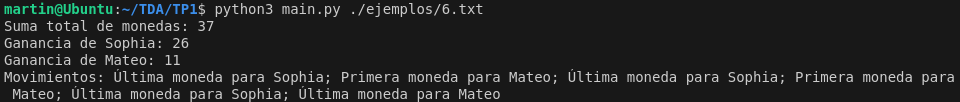
\includegraphics[scale = 0.45]{ {./images/ejemplo_ejecucion_6_monedas} }

Veamos la ejecución de otros ejemplos brindados por la cátedra, por ejemplo el de 20 monedas:

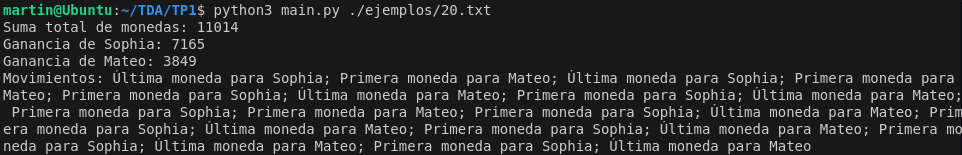
\includegraphics[scale = 0.45]{ {./images/ejemplo_ejecucion_20_monedas} }

Otro ejemplo de la cátedra, el de 100 monedas:

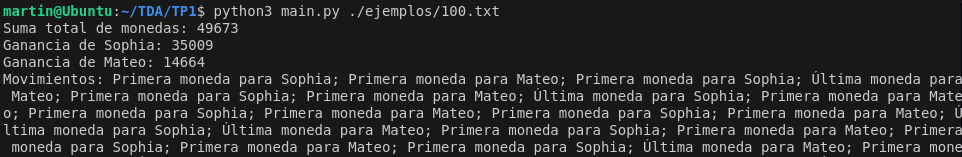
\includegraphics[scale = 0.45]{ {./images/ejemplo_ejecucion_100_monedas} }

Como podemos observar, los resultados obtenidos coinciden con los \textit{Resultados esperados} compartidos por la cátedra.